
	\subsubsection{Dyna-Q}
		
		
\paragraph{}Asumamos que tenemos un modelo del ambiente, esto es, que podemos predecir el siguiente estado y la recompensa dado un estado y una acci�n. La predicci�n puede ser un conjunto de posibles estados con su probabilidad asociada o puede ser un estado que es muestreado de acuerdo a la distribuci�n de probabilidad de los estados resultantes. Dado un modelo, es posible hacer planificaci�n. Lo interesante es que podemos utilizar los estados y acciones utilizados en la planificaci�n tambi�n para aprender. De hecho al sistema de aprendizaje no le importa si los pares estado-acci�n son dados de experiencias reales o simuladas. Dado un modelo del ambiente, uno podr�a seleccionar aleatoriamente un par (estado,acci�n), usar el modelo para predecir el siguiente estado, obtener una recompensa y actualizar valores Q. Esto se puede repetir indefinidamente hasta converger a Q\*.

\paragraph{}El algoritmo Dyna-Q combina experiencias con planificaci�n para aprender m�s r�pidamente una pol�tica �ptima.
La idea es aprender de experiencia, pero tambi�n usar un modelo para simular experiencia adicional y as� aprender m�s r�pidamente 

\paragraph{}El algoritmo de Dyna-Q selecciona pares estado-acci�n aleatoriamente de pares anteriores. Sin embargo, la planificaci�n se puede usar mucho mejor si se enfoca a pares estado-acci�n espec�ficos. Por ejemplo, enfocarnos en las metas e irnos hacia atr�s o m�s generalmente, irnos hacia atr�s de cualquier estado que cambie su valor.Los cambios en las estimaciones de valor V o Q pueden cambiar, cuando se est� aprendiendo o si el ambiente cambia y un valor estimado deja de ser cierto.

\paragraph{}Veamos el pseudoc�digo:
		
		\begin{figure}[h!]
			\centering
			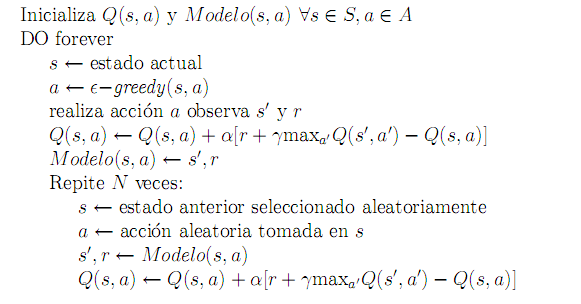
\includegraphics[width=0.6\textwidth]{Dyna.png}
			\caption{Algoritmo Dyna-Q}
		\end{figure}

\paragraph{}En nuestro casos los valores utilizados fueron:

\begin{\begin{itemize}
	
	\item N = 50 
	\item LEARNING\_RATE $= \alpha = 0.8 $
	\item DISCOUNT\_FACTOR $= \delta = 0.95 $
\end{itemize}	
	